\newpage
\subsection{Mechanical Design} \label{Mechanical_Design}
\label{sec:mechanical-design}

\subsubsection{Structure}
\label{sec:4.4.1}
The experiment itself has only two components that are placed inside the gondola. Firstly, the electronics box and then the gimbal on which the telescope is mounted. We require the gimbal to be placed at the edge of the gondola so that the telescope setup is stowed during launch and descent, but still capable of being deployed and performing its required range of motion for observing astronomical targets outside of the gondola.

\begin{figure}[H]
    \centering
	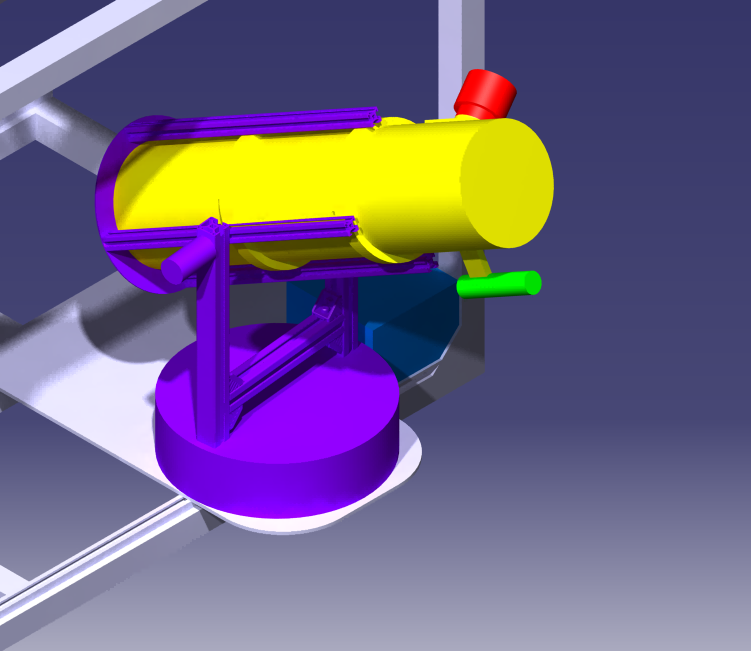
\includegraphics[scale=1.2]{4-experiment-design/img/mechanical/Assembly_v3iso.png}
	\caption{\hl{Overview of experiment structure. Image updated}}
\end{figure}
\subsubsection{Electronics box}
\label{sec:4.4.2}
The electronics box has a dimension 10x10x10 cm which is placed directly inside the gondola. It is estimated to weigh 1.5 kg. The box is made of aluminium side plates with a thick layer of styrofoam placed on the inside of the aluminium plates which protects the electronics. The box has rubber cushion feet that acts as a shock absorber and also thermal insulator from the gondola.

\subsubsection{Gimbal}
\label {sec:4.4.3}

\begin{figure}[h!]
\centering
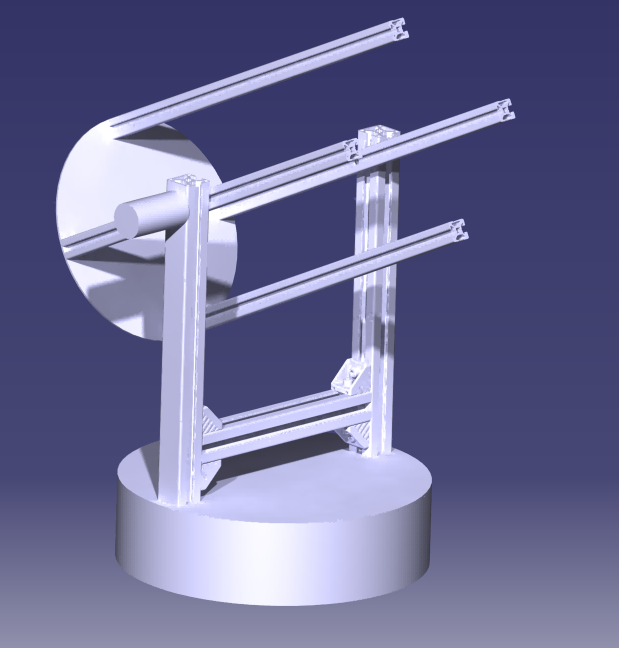
\includegraphics[scale=1]{4-experiment-design/img/mechanical/Aluminium_Gimbal1.png}
\label{fig::mechanical::AlGim}
\caption{\hl{Aluminium Gimbal proposed design (New Image)}}
\end{figure}
\st{We intend to use a three axis gimbal so that we have a maximum field of view. We use CFRP to manufacture the gimbal.} \hl{Aluminium extrusions will be used in order to have an easy manufacturing and adjusting of the structure. Simple ball bearings will be used for the X and Y axes rotations, for the Z axis, a set of two bearings; a ball bearing and a thrust bearing, will be used in order to provide more stability, they will be placed inside the cylindrical cover in the bottom of the gimbal along with the motor in order to provide proper support. The movement of each axis is shown in section 4.8.4 in figure $\ref{fig::software::Yaw_Pitch_Roll}$. The only gearbox expected to be used is the one included with the motors with a reduction gear ratio of 312:1. } The gimbal along with telescope is estimated to weigh around 10kg.



\subsubsection{Fixing interface}
\label {sec:4.4.5}
The telescope itself has certain fixture points and as such, the gimbal will be designed with matching fixture points.\st{ The gimbal is directly fixed on the gondola}\hl{A mounting plate will be fixed to the gondola using a simple aluminium frame attached to the rails of the Gondola.}The gimbal along with the fixing points will first be tested with Finite Element Analysis (FEA) in order to ensure that the whole structure can withstand the loads indicated in the BEXUS manual.
